% use koma script classes
\documentclass[12pt]{scrartcl}

% fix for oliver: https://www.tug.org/pipermail/tex-live/2016-July/038985.html
\makeatletter
\DeclareOldFontCommand{\rm}{\normalfont\rmfamily}{\mathrm}
\DeclareOldFontCommand{\sf}{\normalfont\sffamily}{\mathsf}
\DeclareOldFontCommand{\tt}{\normalfont\ttfamily}{\mathtt}
\DeclareOldFontCommand{\bf}{\normalfont\bfseries}{\mathbf}
\DeclareOldFontCommand{\it}{\normalfont\itshape}{\mathit}
\DeclareOldFontCommand{\sl}{\normalfont\slshape}{\@nomath\sl}
\DeclareOldFontCommand{\sc}{\normalfont\scshape}{\@nomath\sc}
\makeatother



% utf8 charset is required for some german characters
\usepackage[utf8]{inputenc}
% required for nicer footer / header
\usepackage{fancyhdr}
% required for diagramms
\usepackage{pgfplots}
% required for code snippets
\usepackage{listings}
\usepackage{color}
% required for german bibliography list entries
\usepackage[german]{babel}

\usepackage{rotating}
\usepackage{amsmath}

\usepackage{pdfpages}
\usepackage{graphicx}

\usepackage{tikz-uml}
\usepackage{adjustbox}
\usepackage{float}


 %% clickable links for references
\usepackage{hyperref}	%% ocgcolorlinks --> color in pdf viewer, but not printed
% \usepackage[ocgcolorlinks]{hypcap}

\hypersetup{
  colorlinks   = true, %Colours links instead of ugly boxes
  urlcolor     = blue, %Colour for external hyperlinks
  linkcolor    = blue, %Colour of internal links
  citecolor    = blue   %Colour of citations
}


% replaces bibtex, as bibtex has no native support for online sources
\usepackage[
	backend=bibtex,
	style=numeric-comp
	]{biblatex}
\makeatletter % se great overlord fix http://tex.stackexchange.com/questions/311426/bibliography-error-use-of-blxbblverbaddi-doesnt-match-its-definition-ve
\def\blx@maxline{77}
\def\maxwidth#1{\ifdim\Gin@nat@width>#1 #1\else\Gin@nat@width\fi}
\makeatother
% add our bibliography source file
\addbibresource{lit.bib}

% define some code colors
\definecolor{dkgreen}{rgb}{0,0.6,0}
\definecolor{gray}{rgb}{0.5,0.5,0.5}
\definecolor{mauve}{rgb}{0.58,0,0.82}

% define the style of code snippets
\lstset{frame=none,
	language=Java,
	aboveskip=3mm,
	belowskip=3mm,
	showstringspaces=false,
	columns=flexible,
	basicstyle={\small\ttfamily},
	numbers=none,
	numberstyle=\tiny\color{gray},
	keywordstyle=\color{blue},
	commentstyle=\color{dkgreen},
	stringstyle=\color{mauve},
	breaklines=true,
	breakatwhitespace=true,
	tabsize=4
	}

% title page (hacky)
%\newcommand{\seauthor}{Michael Watzko \newline{}und Oliver Wasser\newline{}und Julian Klissenbauer}
\newcommand{\lastModified}{13. Dezember 2016}
\newcommand{\lab}{Projekt Softwaretechnik}
\newcommand{\labtitle}{FlowDesign}
\newcommand{\figurewidth}{0.66\textwidth}

\title{
	~\\ ~\\
	\labtitle
	~\\ ~\\
		\LARGE \textnormal{
     	\lab
	~\\ Wintersemester 2016 ~\\ ~\\
	}
	\begin{figure}[h!]
		\centering
		
\includegraphics[width=.25\textwidth]{../javafx/src/main/resources/images/realIcon.png}
	\end{figure}
}

\subtitle{
\Large \textnormal{
%	~\\ ~\\
%	\textbf{Hausarbeit} \\
~\\
	Studiengang ~\\
	Softwaretechnik und Medieninformatik \\
~\\
	~\\ \large %\lastModified
	}
}

\author{
	\large \textbf{Michael Watzko} (749567) \\
	\large \textbf{Oliver Wasser} (749384) \\
	\large \textbf{Julian Klissenbauer-Mathä} (749564)
}

\date{}

% page header and footer
\pagestyle{fancy}
\lhead{\small Hochschule Esslingen \\ Fakultät Informationstechnik}
%\rhead{\small \lab \\ \labtitle}
\rhead{\small \labtitle}
\lfoot{\small Michael Watzko, Oliver Wasser,\newline{}Julian Klissenbauer-Mathä}
\rfoot{\small Stand: \lastModified}

\newcommand{\textFlowDesign}{FlowDesign}

\newcommand{\textPrincipleSingleResponsibility}{Single-Responsibility-Prinzip}
\newcommand{\textPrincipleLiskovSubstitution}{Liskovsches Substitutionsprinzip}
\newcommand{\textPrincipleOpenClosed}{Open-Closed-Prinzip}
\newcommand{\textPrincipleInterfaceSegregation}{Interface-Segregation-Prinzip}
\newcommand{\textPrincipleDependencyInversion}{Dependency-Inversion-Prinzip}

\newcommand{\textModCore}{Modul Core}
\newcommand{\textModData}{Modul Data}
\newcommand{\textModDataUI}{Modul Data-UI}
\newcommand{\textModJavaFX}{Modul JavaFX}
\newcommand{\textModModel}{Modul Model}
\newcommand{\textModStorage}{Modul Storage}


\newcommand{\textMeetingFirst}{Protokoll zum Kundentreffen am 13. Dezember 2016}
\newcommand{\textMeetingSecond}{Protokoll zum Kundentreffen am 22. Dezember 2016}

\newcommand{\textFlowElements}{Elemente}
\newcommand{\textFlowNotation}{Notation}

\newcommand{\refShort }[1]{\ref{#1}}
\newcommand{\refShortP}[1]{(\ref{#1})}
\newcommand{\refLong} [1]{#1 \ref{#1}}
\newcommand{\refLongP}[1]{#1 (\ref{#1})}


% actual start of the document
\linespread{1.2}
\begin{document}
	\maketitle
	\tableofcontents
	
	\clearpage
	
\section{Einleitung}

Für das Konstruieren benötigt jeder Ingenieur ein strukturiertes Vorgehen. \textFlowDesign{}
soll genau dort unterstützend wirken.
Zusammen mit der Firma IT-Designers GmbH hat sich unser Team im Wintersemester 2016/17 im
Rahmen des Projekts Softwaretechnik an die Entwicklung eines Programms, das diesen Ansatz
nutzt, gewagt.

\subsection{Motivation}
Wie erwähnt entstand das Projekt \textFlowDesign{} im Modul ''Projekt Softwaretechnik'' im vierten Semester des Studiengangs Softwaretechnik und Medieninformatik. \\
Um zu Erfahren wie anspruchsvolle Entwicklungs- und Projektarbeit aussieht, erschien uns dieses Projekt als genau richtig. Es bietet ein relativ offenes Themenfeld, was großen Handlungsspielraum zulässt um unsere gewählten Entwicklungsansätze in der Praxis testen zu können. Daraus erhoffen wir uns unsere Fähigkeiten, sei es in der Entwicklung, Planung und generellen Zusammenarbeit mit dem Kunden oder im Team, weiterentwickeln zu können.


\subsection{Rollenverteilung}
Die Rollenverteilung für das Projekt sah dabei wie folgt aus:

%~\\
\begin{center}
	\begin{tabular}{l|l l}
		Kevin Erath & Kunde     & IT-Designers \\
		Öhmer Haybat & Betreuer & IT-Designers \\
		Andreas Rössler & Betreuender Professor & HS-Esslingen \\
		\\
		Oliver Wasser             & Projektmanager und Dokumentation & \\
		Julian Klissenbauer-Mathä & Chefentwickler & \\
		Michael Watzko            & Entwickler, Qualitätsmanager  \\
		                          & und Dokumentation \\
	\end{tabular}
\end{center}

\pagebreak
\section{Umsetzung}

\subsection{Entwicklungsansatz}
Wir haben uns entschieden eine völlig neue Entwicklung zu beginn, da uns die gewählte
Programmiersprache des vorherigen Teams, welches sich mit \textFlowDesign{} beschäftigte,
nicht zugesagt hatte. Mit Java glauben wir Vorteile etwa im Bezug auf 
Plattformunabhängigkeit zu haben, welche mit C\# und dem .NET-Framework nur schwer zu
realisieren wären. \newline
Unsere Implementierung ist demnach in Java geschrieben und benutzt das UI-Toolkit JavaFX
für die Gestaltung der Oberfläche. \newline
Einzig das Konzept des UI wurde von uns grob dem vorherigem Team nachempfunden.

\subsection{Versionsverwaltung}
Für die Versionverwaltung haben wir uns für Git entschieden. Hierbei haben wir auf einen
bereits bestehenden, eigenen Git-Server auf Basis von Gitblit gesetzt. Hierdurch hatten
wir zu jeder Zeit einen Überblick über die Aktivitäten an der Repository und konnten
uns schnell über die letzten Änderungen informieren.

\subsection{Entwicklungsumgebung}
Als Entwicklungsumgebung haben wir IntelliJ IDEA eingesetzt. Nichtsdestotrotz wurde das Projekt
als Maven-Projekt erstellt, wodurch die Maven-Ordnerstruktur als Grundaufbau verwendet wurde.
Auch alle Abhängigkeiten wurden durch Maven aufgelöst. Somit ist es grundsätzlich möglich das
Projekt auch ohne Entwicklungsumgebung zu übersetzen und auszuführen.

\subsection{Lizenz}
Um zukünftigen Teams, die sich mit der gleichen Aufgabe beschäftigen, eine Grundlage zu geben
haben wir uns dazu entschlossen den Quelltext unter der GPL Lizenz zu veröffentlichen. Zudem
wird der Code jederzeit online abrufbar sein.

	\clearpage
	
\section{\textFlowDesign}

Bei \textFlowDesign{} handelt es sich um eine Methodik, welche dem Entwickler helfen soll
im Voraus saubere Software zu entwerfen. Dabei hilft \textFlowDesign{} etwa bei der
Vermeidung von Abhängigkeiten innerhalb eines Programms durch Entkopplung in einzelne
Module, was ansonsten zu Problemen führen kann.
Datenflüsse werden betrachtet und passende Schnittstellen definiert.

\subsection{System-Umwelt Diagramm}
Beim System-Umwelt Diagramm handelt es sich um eine Betrachtung eines gegebenen oder geplanten Systems, in welcher Interaktionen mit anderen Systemen, Ressourcen und/oder Aktoren dargestellt werden können. Ergänzend hierzu wurde vom Kunden gewünscht, dass bei Interaktionen genauere Details in Listenform hinzugefügt werden können.
Wie im \refLongP{\textMeetingFirst} aufgezeichnet, sollen die einzelnen Interaktionen in der Liste auch mit den passenden Stellen der anderen Diagrammtypen verlinkt sein.


\subsection{Maskenprototyp}
Der Maskenprototyp ist besonders wichtig, um eine grobe Vorstellung zu geben wie das fertig Programm in etwa auszusehen hat. Dieser wird idealerweise in interaktiver Zusammenarbeit, etwa in Kundengesprächen, erstellt. Dabei wurde von unserem Kunden gewünscht, dass bewusst nur rudimentäre Oberflächen erstellbar sind. Damit soll verhindert werden den Eindruck zu vermitteln, dass das Programm bereits fertiggestellt sei.

\subsection{Fluss Diagramm}

Beim Fluss Diagramm wird der Ablauf eines Algorithmus dargestellt. Ein Ablauf kann für sich alleine stehen, oder
anhand des Namens mit einer Aktion eines Maskenprototyp oder als teil eines anderen Algorithmus verknüpft werden.
Ein Flow Diagramm besteht aus Operationen die aneinander gereiht sind, dabei ist das Ergebnis einer Operation der
Parameter für die nächste Operation.
Im folgenden wird auf die Operationen und auf die Notation eingegangen die mit diesem Projekt dargestellt werden kann.
Als Grundlage hat hierbei das ''CheatSheet Flow Design''\cite{flowDesign} gedient. Zuerst werden die einzelnen
Elemente erläutert \refShortP{\textFlowElements} und anschließend die Notation erklärt
\refShortP{\textFlowNotation}.

\subsubsection{\textFlowElements}
\label{\textFlowElements}

Ein Fluss Diagramm hat immer ein Anfang (kleiner Kreis ohne Text) und ein Ende (kleiner Kreis mit X), zwischen dem
die Operationen aufgeführt werden.
\begin{figure}[H]
	\centering
	
\includegraphics[width=\maxwidth{.9\textwidth}]{Element_Start_End.png}
	\caption{Start-Element links, End-Element rechts}
\end{figure}


Eine Operation ist ein größerer Kreis mit dem Namen oder Beschreibung der hier auszuführenden Operation
\begin{figure}[H]
	\centering
	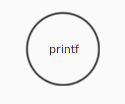
\includegraphics[width=\maxwidth{.9\textwidth}]{Element_Operation.png}
	\caption{Operation-Element}
\end{figure}

Eine Operation kann auch einen Zustand speichern, der über weitere Aufrufe hinweg persistent ist. Dabei wird 
ein Container in die untere rechte Ecke gezeichnet. Dem Zustand kann auch ein Name gegeben werden.
\begin{figure}[H]
	\centering
	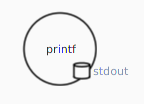
\includegraphics[width=\maxwidth{.9\textwidth}]{Element_Operation_Zustand.png}
	\caption{Operation-Element mit Zustands variable}
\end{figure}

Falls eine Operation auf eine Ressource zugreift, wird dies durch ein Dreieck in der unteren rechten Ecke gezeichnet.
Auch die Ressource kann benannt werden.
\begin{figure}[H]
	\centering
	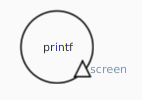
\includegraphics[width=\maxwidth{.9\textwidth}]{Element_Operation_Resource.png}
	\caption{Operation-Element mit Ressourcenzugriff}
\end{figure}

Ein Split-Element stellt die Aufteilung des Programmflusses dar. Das Element wird durch ein Viereck dargestellt
unter dem eine Bezeichnung geschrieben werden kann.
\begin{figure}[H]
	\centering
	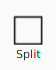
\includegraphics[width=\maxwidth{.9\textwidth}]{Element_Split.png}
	\caption{Split-Element}
\end{figure}

Zum zusammenführen eines Programmflusses wird ein Verbindungselement benötigt. Dies ist ein Strich bei dem
mehrere Flüsse (Abbildung \ref{flowElementVerbindung} links) wieder zu einem zusammengeführt werden (Abbildung
\ref{flowElementVerbindung} rechts).
\begin{figure}[H]
	\centering
	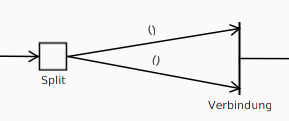
\includegraphics[width=\maxwidth{.9\textwidth}]{Element_Split_Verbindung.png}
	\caption{Verbindungs-Element mit Beispiel}
	\label{flowElementVerbindung}
\end{figure}

Zugriffe auf das Client-System (UI, GUI, WebService, etc \cite{flowDesign}) werden durch ein Portal dargestellt.
Ein Portal ist auch ein Viereck, bei dem sich die Bezeichnung jedoch in dem Viereck befindet. Falls das Fluss Diagramm
von einem Client-System verwendet wird, wird auch das Start und Ende Element durch ein Portal dargestellt.
\begin{figure}[H]
	\centering
	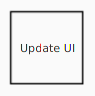
\includegraphics[width=\maxwidth{.9\textwidth}]{Element_Portal.png}
	\caption{Portal-Element}
\end{figure}

Die einzelnen Elemente werden durch Pfeile verbunden auf denen die Übergabedatentypen geschrieben werden. Eine genauere
Erklärung für die Notation kann \refShort{\textFlowNotation} gefunden werden. Optional kann auch an jede beliebige Stelle
eine Kommentarbox eingefügt werden.
\begin{figure}[H]
	\centering
	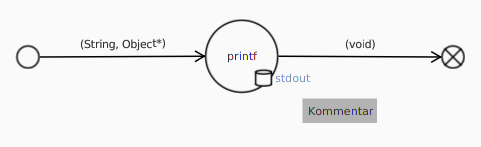
\includegraphics[width=\maxwidth{.9\textwidth}]{Element_connected_comment.png}
	\caption{Beispielhafte Verknüpfung mit Kommentarbox}
\end{figure}

\subsubsection{\textFlowNotation}
\label{\textFlowNotation}	
	
	\clearpage
	\section{Anforderungen}
Hervorgehend aus der Präsentation durch IT-Designers und unseren eignen Vorstellungen zum Projekt haben wir folgende Requirements ausgearbeitet:

\subsection{Funktionale Anforderungen}

\subsubsection{Diagramme}
\begin{itemize}
	\item System-Umwelt-Diagramme
	\item Maskenprototypen
	\item Flow Diagramme
\end{itemize}

\subsubsection{Plattformunabhängigkeit}
\begin{itemize}
	\item Durch Entwicklung in Java auf Windows, Mac OS und anderen Unix-Systemen lauffähig
\end{itemize}

\subsubsection{Projektbasiertes Arbeiten}
\begin{itemize}
	\item Möglichkeit zum Erstellen von Diagrammen innerhalb eines Flow-Projektes, einfaches importieren/exportieren bzw. abspeichern von Projekten
\end{itemize}

\subsubsection{Verlinkbarkeit}
\begin{itemize}
	\item Programmablauf für z.B. einen Button im Maskenprototyp kann in den anderen Diagrammarten dargestellt werden und wird automatisch verlinkt 
\end{itemize}

\subsubsection{Einhaltung von Verknüpfungslogiken}
\begin{itemize}
	\item Automatische Überprüfung auf Korrektheit der Verknüpfungen wie etwa innerhalb eines System-Umwelt-Diagramms, Blockierung von falschen Verbindungen  
\end{itemize}

\subsubsection{Codegenerierung (optional)}
\begin{itemize}
	\item Bei Erfüllung oben genannter Requirements innerhalb des Projektplans: Implementierung von einfacher Codegenerierung aus den erstellten Diagrammen innerhalb eines Projektes
\end{itemize}
	
\subsection{Nicht-Funktionale Anforderungen}

\subsubsection{Aussehen und Handhabung}
Die Oberfläche soll leicht verständlich und intuitiv bedienbar sein.

\subsubsection{Fehlertolleranz bzw. Fehlerabsicherung}
Wenn der Benutzter falsche bzw. ungültige Eingaben macht, so soll dieser darauf hingewiesen werden.

\subsubsection{Skalierbare Darstellung}
Die Anwendung sollte soll sowohl bei Auflösungen wie 1024x768 als auch bei Auflösungen wie 1920x1080 korrekt
dargestellt werden. Zudem soll die Darstellung auf Retina-Displays bzw. im Allgemeinen bei aktivierter
Oberflächenskalierung fehlerfrei sein.

	
	\clearpage
	
\section{Projektplan}
\subsection{Implementierung - 25.10.16 - 12.12.16}
\begin{itemize}
\item Versioning mit Git
\item Implementierung der GUI mit JavaFX
\item Implementierung der Verknüpfungslogik und Bedingungen
\item Implementierung des persistenten Speichers
\end{itemize}

\subsection{Abnahme IT-Designers - 13.12.16 - 23.12.16}
\begin{itemize}
\item Treffen mit dem Kunden
\item Fehlerkorrekturen
\item Kleinere Anpassungen und Ergänzungen
\end{itemize}

\subsection{Abschlusspräsentation - 02.01.17 - 10.01.17}
\begin{itemize}
\item Erstellen der Präsentation
\item Ergänzen der Dokumentation
\end{itemize}

\subsection{Repository Übergabe - 10.01.17}
\begin{itemize}
\item Übergabe der Repository an den Kunden
\end{itemize}
	
	\clearpage
	\section{\textMeetingFirst}
	\label{\textMeetingFirst}
	\begin{figure}[h!]
		\centering
		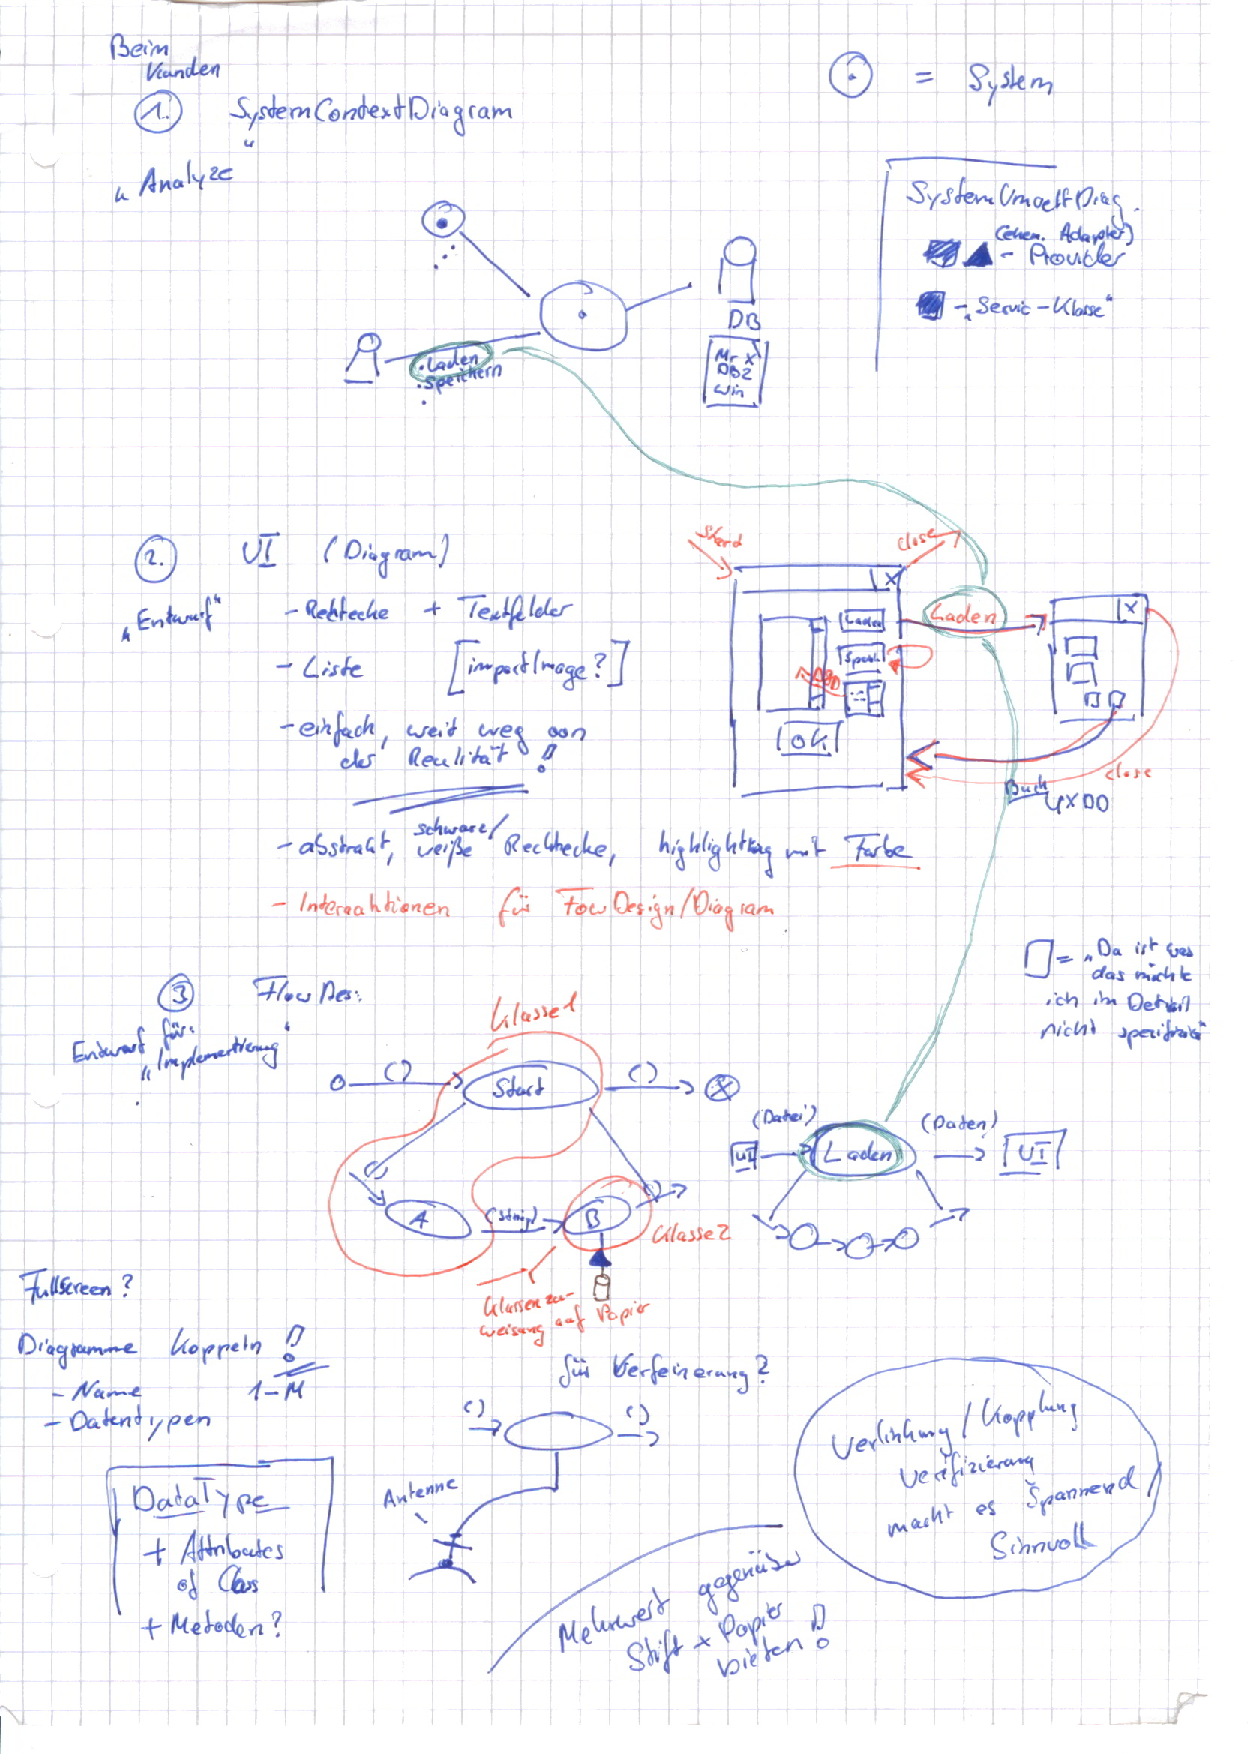
\includegraphics[width=0.95\textwidth]{meeting_2016-12-13.pdf}
	\end{figure}
	
	\clearpage
	\section{\textMeetingSecond}
	\label{\textMeetingSecond}
	\begin{figure}[h!]
		\centering
		\includegraphics[page=1,width=0.95\textwidth]{meeting_2016-12-22.pdf}
	\end{figure}  	
	
	\begin{figure}[h!]
		\centering
		\includegraphics[page=2,width=0.95\textwidth]{meeting_2016-12-22.pdf}
	\end{figure}  		
	
	\clearpage
	
\newcommand{\depBox}[1]{
	\begin{adjustbox}{minipage=0.90\textwidth,margin=0 \smallskipamount,center}
		Abhängigkeiten:	 #1
	\end{adjustbox} ~\\
}

\section{Module}
\subsection{Modulübersicht}
Die Teilbereiche des Projekts wurden in verschieden Module aufgeteilt.

\begin{figure}[h!]
	\centering
	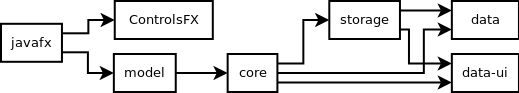
\includegraphics[width=.8\textwidth]{module_dependencies.png}
	\caption{Abhängigkeitsgraph der Module}
	\label{mod_dep_view}
\end{figure}

Der in Abbildung \ref{mod_dep_view} gezeigte Graph enthält keine Abhängigkeiten nach JUnit und
dem JDK aus Gründen der Übersicht. Zudem ist ControlsFX \cite{controlsfx} kein eigen
entwickeltes Modul und wird lediglich aus gründen der Vollständigkeit aufgeführt.

Anzumerken ist auch, dass bis in das \refLongP{\textModCore} keine Abhängigkeiten
gegenüber einer UI-Bibliothek existieren. Das Modul \hyperref[mod_data-ui]{Data-UI} stellt
zwar Komponenten bereit, die für die Integration in eine Benutzeroberfläche benötigt werden,
bleibt jedoch Benutzeroberflächenunabhängig.


\subsection{\textModCore}
\label{\textModCore}
\begin{figure}[h!]
	\centering
	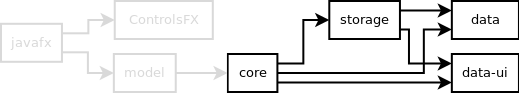
\includegraphics[width=.8\textwidth]{module_dependencies_core.png}
\end{figure}
\depBox{\refLongP{\textModData}, \refLongP{\textModDataUI}, \refLongP{\textModStorage}}

Modulerklräung hier
Core inklusive Abhängigkeiten enthalten alle Logik. Falls eine ander Benutzeroberfläche erstellt,
oder die Logik anderweitig benötigt wird, sollte auf dieses Modul die Abhängigkeit aufgebaut werden.




\subsection{\textModData}
\label{\textModData}
\begin{figure}[h!]
	\centering
	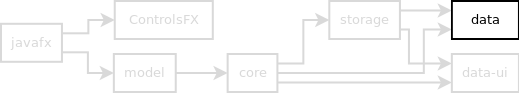
\includegraphics[width=.8\textwidth]{module_dependencies_data.png}
\end{figure}
\depBox{Keine}

Das Modul \textit{data} enthält die Haupt-Geschäftslogik und alle Datenmodelle. Da viel Logik nur darin besteht
die referentielle Integrität bzw. Vollständigkeit der Daten zu gewährleisten ist dieses Modul im Gegensatz zum
Modul \textit{core} relativ schwergewichtig.

\subsubsection{Flow Notation Parser}
Dieser Parser ist für die Umsetzung von textueller Flow-Notation in eine auswertbare Form zuständig. Hierbei können
beispielsweise folgende Konstruke verarbeitet werden:

\begin{itemize}
	\item \{name:string\}
	\item \{int\}
	\item \{(name:string, amount:int)\}
	\item (name:string)
	\item (float)*
	\item (float*, int)
	\item (float*, int)/(double*, int)
\end{itemize}
Vom Parser wird ein generisches \textit{FlowAction} Objekt zurückgegeben, wenn der Vorgang erfolgreich war. Dieses
Objekt kann eines der folgenden Klassen sein:

\begin{itemize}
	\item MultiStream ( \textbf{\{}test\textbf{\}} )
	\item Tupel ( \textbf{(}test\textbf{)} )
	\item Type ( \textbf{name:test} )
	\item Chain ( \textbf{test/int} )
\end{itemize}
Objekte dieser Klassen enthalten entsprechend Möglichkeiten auf die Kind-Elemente (wenn vorhanden) oder
Eigenschaften zuzugreifen.
\subsection{\textModDataUI}
\label{\textModDataUI}
\begin{figure}[h!]
	\centering
	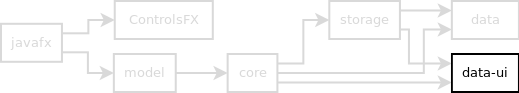
\includegraphics[width=.8\textwidth]{module_dependencies_data-ui.png}
\end{figure}
\depBox{Keine}

Im Modul \textit{data-ui} befinden sich Datenmodelle, die nicht direkt in die eigentliche Geschäftslogik
eingebaut werden können / sollen, sondern eigentlich nur für die Oberfläche selbst benötigt werden.

Ein Beispiel hierfür ist das Changelog, welches beim Start der Anwendung geöffnet werden kann.
Sollte in Zukunft beispielsweise die Möglichkeit eingebaut werden, Oberflächeneinstellungen zu speichern, 
so wäre das Modul \textit{data-ui} der entsprechende Platz für die Datenmodelle.

\subsection{\textModJavaFX}
\label{\textModJavaFX}
\begin{figure}[h!]
	\centering
	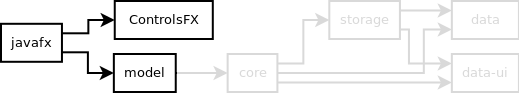
\includegraphics[width=.8\textwidth]{module_dependencies_javafx.png}
\end{figure}
\depBox{\refLongP{\textModModel}, ControlsFX (ext. \cite{controlsfx})}

Modulerklräung hier




\subsection{\textModModel}
\label{\textModModel}
\begin{figure}[h!]
	\centering
	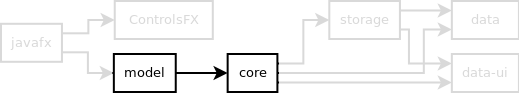
\includegraphics[width=.8\textwidth]{module_dependencies_model.png}
\end{figure}
\depBox{\refLongP{\textModCore}}

Dieses Modul wurde erst spät im Entwicklungsprozess mit einbezogen und beinhaltet bisher noch keine Klassen.
Es ist allerdings dafür vorgesehen, Klassen zu enthalten, die für die Oberfläche gebraucht werden, allerdings
unabhängig vom verwendeten Windowing-Toolkit sind.




\subsection{\textModStorage}
\label{\textModStorage}
\begin{figure}[h!]
	\centering
	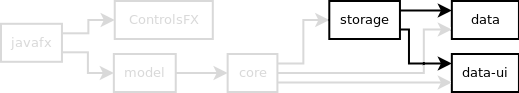
\includegraphics[width=.8\textwidth]{module_dependencies_storage.png}
\end{figure}
\depBox{\refLongP{\textModData}, \refLongP{\textModDataUI}}

Das Storage Modul enthält sowohl eine abstrake Definition von \textit{Serializern} und \textit{StorageHandlern}
als auch eine Implementation für XML inklusive \textit{Serializer} für Komponenten in \refLongP{\textModData} und
\refLongP{\textModDataUI}.

\subsubsection{StorageHandler}
Die Klasse \textit{StorageHandler} ist hält \textit{Storage}s und verteilt Serialisierungsaufgaben an
das entsprechende \textit{Storage} anhand eines Textidentifikators (für XML lautet dieser 'xml').
Eine weitere \textit{Storage} Implementation kann anhand eines neuen Textidentifkators registriert werden,
wodurch ein Umstieg von XML auf JSON, SQL oder eine andere Implementation vereinfacht wird.

\subsubsection{Storage}
Ein \textit{Storage} stellt ein Speicherort für alle zum Projekt gehörenden Komponenten dar. Je nach
Implementation kann dies XML (implementiert), JSON, SQL oder andere sein (nicht implementiert). Bei einem
\textit{Storage} können \textit{Serializer} für weitere Komponenten registriert werden. Sowohl Lese- als
auch Schreibhandles und Hilfsklassen für die \textit{Serializer} werden über Generics in \textit{Storage}
definiert.

\subsubsection{Serializer}
Ein \textit{Serializer} hat die Aufgabe eine Komponente zu serialisieren und wieder zu deserialisieren.
Der Umfang eines \textit{Serializer}s sollte sich auf eine Komponente beziehen (siehe \refLong{\textPrincipleSingleResponsibility}).
	
	\clearpage
	
\section{Einhaltung Programmierkonzepte}

Programmierprinzipien sind essentiell für die Wartbarkeit, Korrektheit und vor allem die Verständlichkeit eines Programmcodes. Die wachsende Komplexität von Programmen und der damit steigende Entwicklungsaufwand erfordern sauberes und strukturiertes arbeiten mehr den je. 


\subsection{SOLID}
Bei SOLID handelt es sich um grundlegende Prinzipien der objektorientierten Programmierung, welche von Robert C. Martin in den frühen 2000ern formuliert wurden.  Alle dieser Prinzipien dienen zur Verbesserung der Wartbarkeit und Erweiterbarkeit von Computerprogrammen. 



\subsubsection{\textPrincipleSingleResponsibility}
\label{\textPrincipleSingleResponsibility}
Das Single-Responsibility-Prinzip besagt, dass eine Klasse, Methode oder Funktion
nur einer Aufgabe verschrieben sein soll. So soll die Funktion zu Berechnung einer
Potenz nur dies tun und nicht gleichzeitig das Ergebnis zbsp auf einer GUI ausgeben.
Dadurch entwickelt sich ein Art Baukastenprinzip bei dem die unterschiedlichen 
Funktionen einfach miteinander verknüpft und oder ausgetauscht werden können, da
keine unnötigen Abhängigkeiten aufgebaut werden. ''Gottklassen'', die viele
verschiedene Funktionalitäten vereinen, sind nicht erlaubt.

\subsubsection{\textPrincipleOpenClosed}
\label{\textPrincipleOpenClosed}
Das Open-Closed-Prinzip besagt, dass eine Klasse, Methode oder Funktion offen
für Erweiterungen aber geschlossen für Veränderungen sein soll. So soll es möglich
sein die Klasse Drucker um ein weiteres Papierformat zu erweitern, jedoch darf sich
das Verhalten von verschiedenen von Drucker abgeleiteten Klassen nicht unterscheiden.

\subsubsection{\textPrincipleLiskovSubstitution}
\label{\textPrincipleLiskovSubstitution}
Das Liskovsche Substitutionsprinzip besagt, dass ein Computerprogramm weiter funktionsfähig bleiben muss, auch wenn Objekte vom Typ T durch Objekte vom Typ S ersetzt werden, wobei S eine Unterklasse von T darstellt (vgl. \cite{wiki:lsp}, Z. 5). Oder kurz gesagt \glqq Subclasses should be substitutable for their base classes\grqq(\cite{knoernschild2002java}, S. 11).

Bei einer solchen Vorgehensweise ist es außerordentlich wichtig, dass das Prinzip \textbf{Design by Contract} eingehalten wird (vgl. \cite{goll2014architektur}, S. 5), damit das Computerprogramm weiterhin richtig funktioniert. Nach außen hin müssen die Operationen beider Klassen in allen Fällen gleich funktionieren.

Die logische Konsequenz dieses Prinzips ist eine verbesserte Erweiterbarkeit und Korrektheit (vgl. \cite{itDesignersSOLID}, S. 2), da Funktionalität relativ einfach angepasst werden kann, ohne bestehenden Code zu verändern. 
Dadurch wird auch das \refLongP{\textPrincipleOpenClosed} impliziert.


\subsubsection{\textPrincipleInterfaceSegregation}
\label{\textPrincipleInterfaceSegregation}
Das Interface Segregation Principle (ISP), oder zu deutsch ''Schnittstellenaufteilungsprinzip'' (\cite{wiki:isp}, Zeile 1), verlangt, dass Schnittstellen jeweils auf einen Aufgabenbereich zugeschnitten sind.
Anstatt einer großen Schnittstelle soll für jeden Aufgabenbereich eine eigene
Schnittstelle definiert werden, die keine Abhängigkeiten zu anderen Teilen des Programms 
aufbaut, die für die eine Aufgabe nicht benötigt werden.
Im Grunde genommen entspricht dies dem  \refLongP{\textPrincipleSingleResponsibility} für Schnittstellen.

Anderen Programmteilen wird dadurch ermöglicht mit Schnittstellen arbeiten zu können, ohne andere nicht benötigte Abhängigkeiten zu bilden: ''Clients [oder andere Programmteile] sollten nicht dazu gezwungen werden, von Interfaces abzuhängen, die sie gar nicht brauchen'' (vgl. \cite{goll2014architektur} S. 10).


\subsubsection{\textPrincipleDependencyInversion}
\label{\textPrincipleDependencyInversion}
Das Dependency Inversion Principle, oder zu deutsch ''Abhängigkeits-Umkehr-Prinzip'' (\cite{wiki:dip}, Zeile 1),
beschreibt das bei hierarchischer Verteilung von Modulen, Module niedrigerer Ebenen von Modulen höherer Ebenen abhängen.
Module höherer Ebenen stellen somit Anforderungen durch Interfaces, die Module niedrigerer Ebenen zu implementieren haben.
Meist sind diese Interfaces dabei in eigene Module aufgeteilt. Die Abhängigkeit ist somit umgekehrt wie traditionell
zuerst zu vermuten sei.

Mit ''höheren Modulen'' sind dabei Module gemeint, die Funktionalität meist weiter abstrahiert haben und auf 
Funktionalität von ''niederen'' - und sehr spezifischen - Modulen aufbauen.

	
	\clearpage
	\section{Aufbau Diagramm-Element}
\subsection{Joint-Group}
Eine Joint-Group ist die Implementierte Art und Weise wie gleichartige Joints gruppiert werden.
Eine solche Gruppe besitzt Maximal- bzw. Minimalzahlen von Joints, wobei neue Joints durch eine
Factory erstellt werden. Alle diese Informationen werden beim Konstruktoraufruf übergeben.
Elemente wie die Operation haben beispielsweise view Joint-Groups. Zwei für Flow- bzw. Abhängigkeits-Eingang
und zwei für Flow- bzw. Abhängigkeits-Ausgang.

\subsection{Joint}
Ein Joint ist ein Verbindungsknoten. Je nach Konfiguration kann ein Joint als Eingang, Ausgang oder beides dienen.
Bisher gibt es sowohl einen \textit{FlowJoint} als auch einen \textit{DependencyJoint}.

\pagebreak
\section{Erweiterung}
Beim Architekturentwurf wurde darauf geachtet das Programm so einfach wie möglich erweiterbar zu machen.
Dieses Kapitel zeigt wie der vorhandene Code erweitert und um Inhalt ergänzt werden kann.

\subsection{Erweiterung um einen Diagrammtyp}
Im Folgenden soll ein neuer Diagramm-Typ mit dem Namen ''Example'' beispielhaft erstellt werden.

\subsubsection{Datenmodell}
Für alle bisherigen Diagramme wurde ein eigenes Paket erstellt. Das ist keine Voraussetzung, hilft allerdings bei der
Strukturierung. Im Folgenden wird deshalb davon ausgegangen, dass das Paket \textit{com.tallbyte.flowdesign.data.example}
verwendet wird.
Hier muss eine Klasse ''ExampleDiagram'' erstellt werden, welche von \textit{Diagram} erbt. Sollte es erwünscht sein,
dass Elemente des Diagramms von einer bestimmten Art sind, so kann dies über den generischen Parameter von 
\textit{Diagram} angegeben werden.

\begin{figure}[h!]
	\centering
	\begin{lstlisting}
public class ExampleDiagram extends Diagram<DiagramElement> {

    public ExampleDiagram(String name) {
        super(name, null);
    }

    public EnvironmentDiagram(String name, DiagramElement root) {
        super(name, root);
    }
}
	\end{lstlisting}
	\caption{Beispiel Diagramm-Klasse}
\end{figure}

\subsubsection{View}
Das Diagramm hat keine eigentliche View. Diese Aufgabe wird direkt von der Klasse \textit{DiagramPane} im Modul 
\textit{javafx} umgesetzt. Hier ist Diagramm-spezifisch nichts zu verändern.

\subsubsection{Handler}
Der \textit{DiagramHandler} ist die Diagramm-spezifische Schnittstelle, die Aufgaben wie die Erstellung von neuen
Diagramm-Instanzen oder die Bereitstellung verfügbarer Properties übernimmt. Zur Vereinfachung gibt es bereits eine
abstrakte Klasse, die die komplexesten Aspekte des Intefaces \textit{DiagramHandler} verbirgt. Diese kann erweitert
werden womit folgende Klasse im Kontext des Beispiels zu erstellen ist.

\begin{figure}[h!]
	\centering
	\begin{lstlisting}
public class ExampleDiagramHandler extends DiagramHandlerBase<ExampleDiagram, DiagramElement, DiagramImage> {

    public ExampleDiagram() {
        addEntries("System", System.class,
                System::new,
                EllipseDiagramImage::new,
                SystemElementNode::new
        );
    }

    @Override
    protected ExampleDiagram createNewDiagramInstance(String name) {
        return new ExampleDiagram(name);
    }
    
    @Override
    public ObservableList<Property<?>> getDiagramProperties(ExampleDiagram diagram) {
        ObservableList<Property<?>> list = super.getDiagramProperties(diagram);

		// add properties

        return list;
    }
}
	\end{lstlisting}
	\label{diagram_handler}
	\caption{Beispiel Diagramm-Handler-Klasse}
\end{figure}
Der Methodenaufruf von \textit{addEntries} wird später noch im Kapitel zum Hinzufügen neuer Diagramm-Element
erklärt (\ref{add_element}). Ansonsten kann in der Methode \textit{getDiagramProperties} eine Liste mit verfügbaren
Properties für ein Diagramm erstellt werden. Diese Liste wird verwendet, um auf der Oberfläche Optionen für das
jeweilige Diagramm einzublenden.
\\r Diagrammtyp
\\
Damit der Handler auch aktiv genutzt wird, muss noch ein Methodenaufruf in der Klasse \textit{DiagramHandler} gemacht
werden.

\begin{figure}[h!]
	\centering
	\begin{lstlisting}
static {
    addHandler(EnvironmentDiagram.class, new EnvironmentDiagramHandler());
    addHandler(FlowDiagram.class, new FlowDiagramHandler());
    addHandler(MaskDiagram.class, new MaskDiagramHandler());
        
    // diese Zeile muss eingefuegt werden
    addHandler(ExampleDiagram.class, new ExampleDiagramHandler());
}
	\end{lstlisting}
	\label{diagram_handler}
	\caption{Diagramm-Handler verfügbar machen}
\end{figure}
\subsubsection{Serialisierung}
Damit der neu-erstellte Diagramm-Typ nun auch gespeichert werden kann muss ein (XML-)Serializer erstellt werden.
\\
// TODO Michael

\subsubsection{Strings}
Da der Projektbaum und andere UI-Elemente automatisch für alle verfügbaren Diagrammtypen erstellt werden müssen
die angezeigten Texte extern verwaltet werden. Hierfür wird das Java-eigene Ressourcensystem verwendet. Im Ressourcen-
Verzeichnis in der Maven-Struktur befindet sich das Resource-Bundle \textit{MessagesBundle}. Hier müssen folgende Strings
bereitgestellt werden:

\begin{itemize}
	\item tree.overview.ExampleDiagram = Example
	\item menu.edit.new.ExampleDiagram = New Example-Diagram...
	\item popup.new.ExampleDiagram.title = New Example Diagram
	\item popup.new.ExampleDiagram.field.name = Name
	\item context.new.ExampleDiagram=New...
\end{itemize}

\pagebreak
\subsection{Erweiterung um ein Diagramm-Element}
\label{add_element}
Im Folgenden soll ein neues Diagramm-Element mit dem Namen ''ExampleElement'' beispielhaft erstellt werden.

\subsubsection{Datenmodell}
// TODO Michael
Zuerst muss das entsprechende Datenmodell erstellt werden. Nach bisheriger Konvention gehören die Diagramm-Elemente
für ein spezielles Diagramm in das gleiche Paket wie die entsprechende Diagramm-Klasse. Das ist allerdings keine
Voraussetzung.

\begin{figure}[h!]
	\centering
	\begin{lstlisting}
public class ExampleElement extends DiagramElement {

    public static final String JOINT_GROUP = "io";

    public ExampleDiagramElement() {
    }

    @Override
    protected Iterable<JointGroup<?>> createJointGroups() {
        return new ArrayList<JointGroup<?>>() {{
            add(new JointGroup<>(System.this, JOINT_GROUP , 4, 4, element -> new DependencyJoint(element, JointType.INPUT_OUTPUT, 0, 0), 4));
        }};
    }

    public JointGroup<?> getJointGroup() {
        return getJointGroup(JOINT_GROUP);
    }

}
	\end{lstlisting}
	\caption{Beispiel Diagramm-Element-Klasse}
\end{figure}
Hier wird ein einfaches Element erstellt, dass eine einzige Joint-Gruppe bereitstellt, die minimal und maximal
vier Joints zur Verfügung stellt, wobei einzelne Joints sowohl als Eingang als auch als Ausgang verwendet werden
können. Zudem ist die Art der Verbindung, welche von den Joints erstellt werden kann eine Abhängigkeitsverbindung
(ein Kreis am Ziel).
\subsubsection{View}
Damit das neue Element später auch auf der Zeichenfläche angezeigt werden kann, muss erst eine View dafür erstellt
werden. Alle View müssen die Basis-Klasse \textit{ElementNode} erweitern. Diese stellt bereits einige wichtig
Funktionen wie das verteilen von Joints auf der Oberfläche oder das vergrößern / verkleinern zur Verfügung.

\begin{figure}[h!]
	\centering
	\begin{lstlisting}
public class ExampleElementNode extends ElementNode<DiagramImage> {

    private final ExampleElement example;

    public SystemElementNode(ExampleElement element, DiagramImage content) {
        super(element, content, Pos.CENTER);

        this.example = element;
    }

    @Override
    protected void setup() {
        super.setup();

        addJointsAcrossCircle(new JointGroupHandler(example.getJointGroup(), 0, 1));
    }
}
	\end{lstlisting}
	\caption{Beispiel Diagramm-Element-Node}
\end{figure}
Durch den Methodenaufruf \textit{addJointsAccrossCircle} werden alle Joints der Joint-Group des übergeben
ExampleElements komplett über den Umfang einer Ellipse verteilt, der sich durch Höhe und Breite des Elements
ergibt. Die \textit{0} steht hier für den Offset im Kreis (Intervall [0;1]), die \textit{1} steht für den
verwendeten Umfang (Intervall [0;1]) in Prozent.
\\
\\
Es stehen hier folgende Funktionen zur Verfügung:
\begin{itemize}
	\item addJointsAccrossRectangle
	\item addJointsAccrossRectangleCentered
	\item addJointsAccrossCircle
	\item addJointsAccrossCircleCentered
\end{itemize}
Der dritte Parameter beim Super-Konstruktoraufruf steht für die Position des Textfelds für den Namen. Gültige
Werte sind \textit{Pos.CENTER} und \textit{Pos.BOTTOM\_CENTER}.

\subsubsection{Image}
Das \textit{DiagramImage} stellt den Teil des Views dar, der für das eigentliche Erscheinungsbild verantwortlich ist,
also z.B. ein Kreis bzw. Oval bei der Operation. Beim Erweitern des DiagramImages muss lediglich die \textit{repaint()}
Methode überschrieben werden. Zusätzlich ist es allerdings auch möglich eigene Properties zu definieren, um das
Verhalten des Images zu steuern (\ref{code_extra_references}).
\begin{figure}[h!]
	\centering
	\begin{lstlisting}
public class ExampleDiagramImage extends DiagramImage {

    public EllipseDiagramImage() {

    }

    @Override
    public void repaint() {
        GraphicsContext context = getGraphicsContext2D();
        double width  = getWidth();
        double height = getHeight();

        context.clearRect(0, 0, width, height);
        context.setStroke(getColor());
        context.setLineWidth(1.5);
        context.strokeOval(
                context.getLineWidth(), context.getLineWidth(),
                width - 2*context.getLineWidth(), height - 2*context.getLineWidth()
        );
    }

}
	\end{lstlisting}
	\label{diagram_handler}
	\caption{Beispiel Diagram-Image}
\end{figure}
\subsubsection{Factory}
Um das neue Element nun endgültig in der Oberfläche verfügbar zu machen muss schlussendlich noch eine Factory
erstellt werden. Dies ist im entsprechenden \textit{DiagramHandler} für den jeweiligen Diagramm-Typ zu machen.
Für Flow-Diagramme also im \textit{FlowDiagramHandler}. In diesem Fall ist es der \textit{ExampleDiagramHandler}.
Hier muss im Konstruktor folgende Zeile eingefügt werden.
\begin{figure}[h!]
	\centering
	\begin{lstlisting}
addEntries("ExampleElement", ExampleElement.class,
        ExampleElement::new,
        ExampleDiagramImage::new,
        ExampleElementNode::new
);
	\end{lstlisting}
	\label{diagram_handler}
	\caption{Beispiel Element Factory}
\end{figure}
Um unnötige Klassen bzw. riesige Code-Konstrukte zu vermeiden werden hier Lambda-Ausdrücke eingesetzt.
\subsubsection{Serialisierung}
// TODO Michael

\pagebreak
\subsection{Weitere Referenzen}
\label{code_extra_references}
Auf Grund der Offenheit des Systems sind eine Vielzahl von Modifikationen möglich, die nicht alle in dieser
Dokumentation behandelt werden können. Allerdings sind bereits einige Beispiele im Programmcode vorhanden.
Die folgende Liste zeigt einige Referenzen für \textit{erweiterte} Funktionen:

\begin{itemize}
	\item Extra Textfeld im View (\textit{OperationalUnitElementNode\#setup()}
	\item Property-Verbindung mit dem Image (\textit{EndElementNode\#EndElementNode()})
\end{itemize}
	
	\clearpage
	
\section{Benutzerhandbuch}

\subsection{Projektauswahlfenster}
Das Programm startet mit einem Auswahlfenster für Projekte. Hier haben Sie die Möglichkeit zuletzt erstellte Projekte zu öffnen, andere existierende Projekte hinzuzufügen oder ein neues Projekt zu erstellen. 

\begin{figure}[h!]
	\centering
	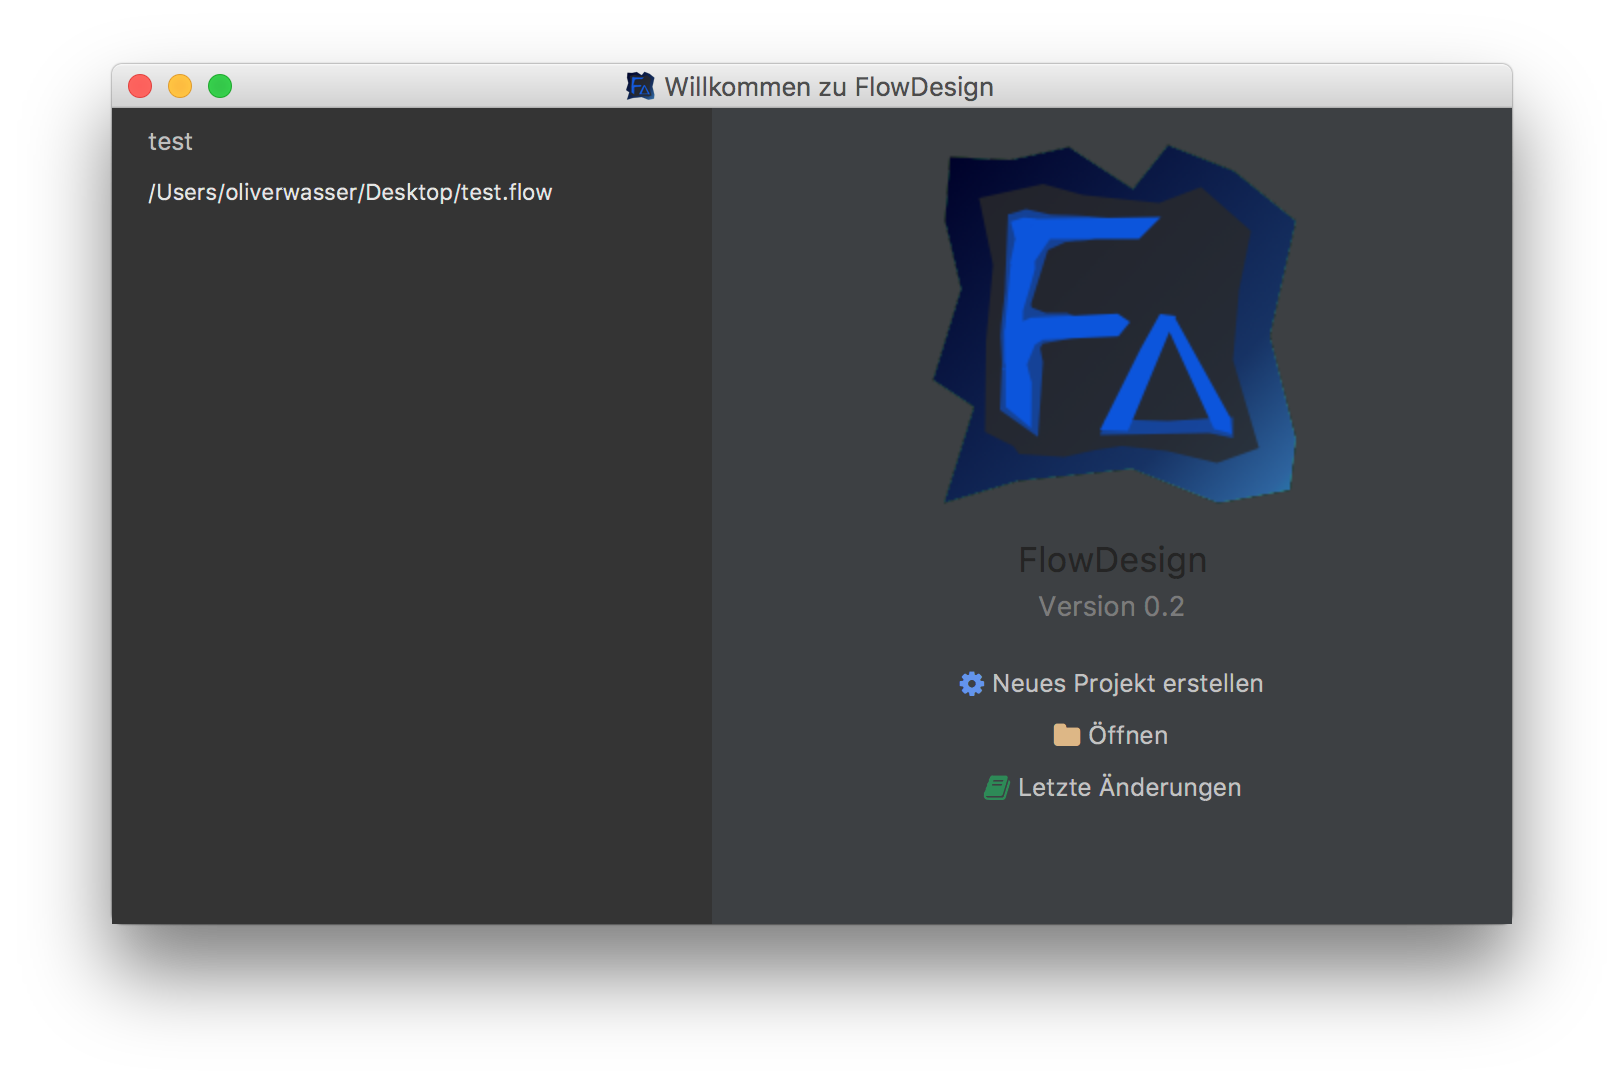
\includegraphics[width=1.0\textwidth]{Auswahlfenster.png}
	\caption{Auswahlfenster}
\end{figure}


\subsubsection{Öffnen eines kürzlich erstellten Projekts}
\begin{itemize}
\item Zum Öffnen eines kürzlich erstellten Projekts, wählen Sie mit einem Doppelklick das gewünschte Projekt im linken Teil des Auswahlfensters. 
\end{itemize}
\subsubsection{Öffnen eines beliebigen Projekts}
\begin{itemize}
\item Zum Hinzufügen eines anderen bestehenden Projektes, wählen Sie mit einem Linksklick ''Öffnen''. Es erscheint ein Fenster zur Auswahl des Dateipfades. Wählen Sie nun das gewünschte Projekt als ''.flow'' Datei aus und bestätigen Sie anschließend mit ''Open''. 
\end{itemize}
\subsubsection{Erstellen eines neuen Projekts}
\begin{itemize}
\item Zum Erstellen eines neuen Projektes, drücken Sie "Neues Projekt erstellen". Im folgenden Fenster tragen Sie einen Name und Speicherort für Ihr Projekt ein. Bestätigen Sie mit ''Ok''.  
\end{itemize}

\subsection{Projektfenster}
\subsubsection{Menüleiste}
\begin{figure}[h!]
	\centering
	
\includegraphics[width=1.0\textwidth]{Leiste.png}
	\caption{Menüleiste unter macOS}
\end{figure}
\begin{itemize}
\item Die Menüleiste enthält die Auswahlpunkte ''Datei'', ''Bearbeiten'', ''Aktion'', ''Diagramm'' und ''Hilfe''.
\item Die für die einzelnen Aktionen nötigen Shortcuts werden Ihnen jeweils zugehörig in der Menüleiste angezeigt. 

\begin{figure}[h!]
	\centering
	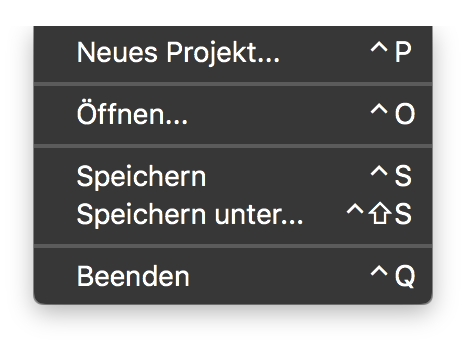
\includegraphics[width=.4\textwidth]{Leiste_Datei.png}
	\caption{Menüleiste - ''Datei''}
\end{figure}

\item Unter ''Datei'' ist es Ihnen möglich ein anderes Projekt zu öffnen, das aktuelle Projekt zu speichern oder mit ''Speichern unter'' eine neue Kopie unter einem beliebigen Pfad abzulegen.

\begin{figure}[h!]
	\centering
	
\includegraphics[width=.4\textwidth]{Leiste_Bearbeiten.png}
	\caption{Menüleiste - ''Bearbeiten''}
\end{figure}

\item Unter ''Bearbeiten'' haben Sie die Möglichkeit neue Diagramme jedes Typen zu erstellen.

\begin{figure}[h!]
	\centering
	
\includegraphics[width=.4\textwidth]{Leiste_Aktion.png}
	\caption{Menüleiste - ''Aktion''}
\end{figure}

\item ''Aktion'' enthält die Suche nach Diagramme. Diese kann ebenfalls mit dem Lupensymbol in der oberen rechten Ecke des Programmes abgerufen werden.

\begin{figure}[h!]
	\centering
	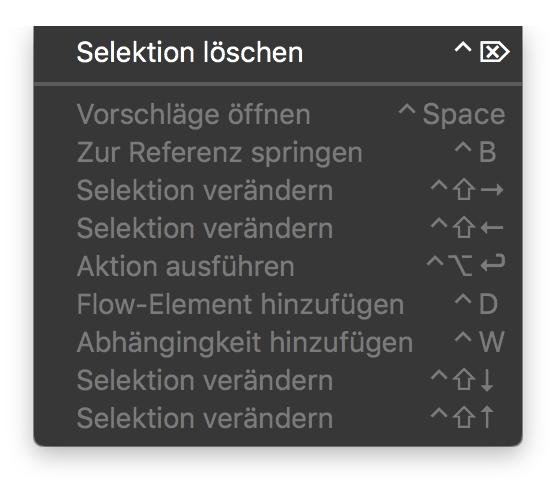
\includegraphics[width=.4\textwidth]{Leiste_Diagram.png}
	\caption{Menüleiste - ''Diagram''}
\end{figure}

\item  Unter ''Diagramm'' finden Sie sämtliche Optionen die das intelligente Arbeiten mit Diagrammen betrifft. Dazu gehört der Quick-Jump in verlinkte Diagramme oder das Hinzufügen von Abhängigkeiten.
\end{itemize}

\begin{figure}[h!]
	\centering
	
\includegraphics[width=.4\textwidth]{Leiste_Hilfe.png}
	\caption{Menüleiste - ''Hilfe''}
\begin{itemize}
\item Wählen Sie ''Hilfe'', um Informationen über den aktuellen Programmbuild zu erhalten.	
\end{itemize}
\end{figure}




\subsubsection{Projektbaum und Anlegen neuer Diagramme}

\begin{figure}[h!]
	\centering
	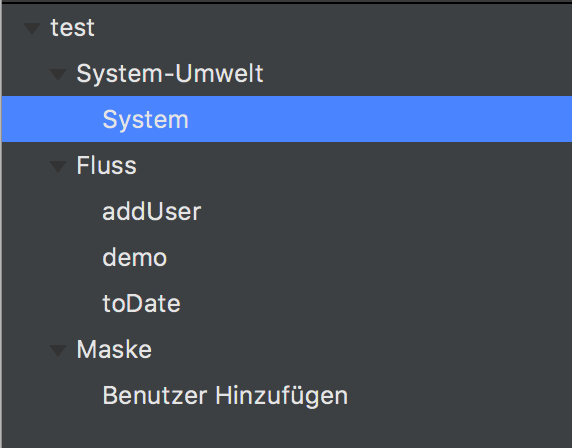
\includegraphics[width=.4\textwidth]{Projektbaum.png}
	\caption{Projektbaum}
\end{figure}

\begin{itemize}
\item Der Projektbaum befindet sich im Programm auf der linken Seite.
\item In der obersten Zeile finden Sie Ihren zuvor gewählten Projektnamen wieder, gefolgt von den drei Diagrammtypen 'System-Umwelt', ‘Fluss‘ und ‘Maske‘. Sie können beliebig viele Diagramme eines Typs erstellen.

\begin{figure}[h!]
	\centering
	
\includegraphics[width=.4\textwidth]{Projektbaum_Erstellen.png}
	\caption{Projektbaum - Erstellen}
\end{figure}

\item Um ein neues Diagramm zu erstellen, drücken Sie mit der rechten Maustaste auf den gewünschten Diagrammtyp. Wählen Sie nun ‘Erstellen' und vergeben Sie einen Namen, beachten Sie dabei das ein Name nur einmalig vergeben werden kann. 
\end{itemize}

\begin{figure}[h!]
	\centering
	
\includegraphics[width=.4\textwidth]{Projektbaum_Bearbeiten.png}
	\caption{Projektbaum - Bearbeiten}
\begin{itemize}	
\item Um bereits erstellte Diagramme zu löschen oder umzubenennen, drücken Sie mit der rechten Maustaste auf das gewünschte Diagramm und wählen Sie die Änderung welche Sie vornehmen möchten. Wenn Sie ein Diagramm umbenennen, wird die Namensänderung durch das Programm automatisch in allen anderen Diagrammen und Referenzen übernommen.
\end{itemize}
\end{figure}




\subsubsection{Zeichenfläche}




\subsubsection{Ändern des Programmdesigns}
\begin{figure}[h!]
	\centering
	
\includegraphics[width=.4\textwidth]{Design_Aendern.png}
	\caption{Designauswahl und Suche}
\begin{itemize}	
\item Das Programm bietet Ihnen die Möglichkeit, zwischen drei verschiedenen Designs zu wählen. Zum Ändern des aktuellen Designs befindet sich im oberen rechten Teil des Fensters eine Designauswahl. Sie haben hier außerdem die Möglichkeit mit Hilfe des Lupensymbols die Suche aufzurufen (ebenfalls über die Menüleiste möglich, siehe 9.2.1).
\end{itemize}
\end{figure}
	
	\clearpage
	\section{Schlusswort}
Abschließend können wir behaupten, dass das ganze Team von diesem Projekt profitiert hat. Zum Einen konnten
wir unser technisches Wissen erweitern, zum Anderen konnten wir den Umgang mit Kunden
	
	\clearpage
	\addcontentsline{toc}{section}{\listfigurename}
	\listoffigures
	
	\clearpage
	\printbibliography[heading=bibintoc]
\end{document}
